\documentclass{beamer}
\usepackage[utf8]{inputenc}
\usetheme{Madrid}
\usecolortheme{default}
\usepackage{amsmath,amssymb,amsfonts,amsthm}
\usepackage{txfonts}
\usepackage{tkz-euclide}
\usepackage{listings}
\usepackage{adjustbox}
\usepackage{array}
\usepackage{tabularx}
\usepackage{gvv}
\usepackage{lmodern}
\usepackage{circuitikz}
\usepackage{tikz}
\usepackage{graphicx}
\setbeamertemplate{page number in head/foot}[totalframenumber]
\usepackage{tcolorbox}
\tcbuselibrary{minted,breakable,xparse,skins}
\definecolor{bg}{gray}{0.95}
\DeclareTCBListing{mintedbox}{O{}m!O{}}{%
  breakable=true,
  listing engine=minted,
  listing only,
  minted language=#2,
  minted style=default,
  minted options={%
    linenos,
    gobble=0,
    breaklines=true,
    breakafter=,,
    fontsize=\small,
    numbersep=8pt,
    #1},
  boxsep=0pt,
  left skip=0pt,
  right skip=0pt,
  left=25pt,
  right=0pt,
  top=3pt,
  bottom=3pt,
  arc=5pt,
  leftrule=0pt,
  rightrule=0pt,
  bottomrule=2pt,
  toprule=2pt,
  colback=bg,
  colframe=orange!70,
  enhanced,
  overlay={%
    \begin{tcbclipinterior}
    \fill[orange!20!white] (frame.south west) rectangle ([xshift=20pt]frame.north west);
    \end{tcbclipinterior}},
  #3,
}
\lstset{
    language=C,
    basicstyle=\ttfamily\small,
    keywordstyle=\color{blue},
    stringstyle=\color{orange},
    commentstyle=\color{green!60!black},
    numbers=left,
    numberstyle=\tiny\color{gray},
    breaklines=true,
    showstringspaces=false,
}
\begin{document}

\title 
{8.2.27}
\date{september 2025}


\author 
{Namaswi-EE25BTECH11060}
\frame{\titlepage}
\begin{frame}{Question}
Find Equation of curve whose Focus is $\brak{0,-3}$ and Directrix y=3
\end{frame}
\begin{frame}{Solution}
 General Equation of a conic is given by\\
\begin{align}
\Vec{x}^\top \Vec{V} \Vec{x} +2 \Vec{u}^\top \Vec{x}+f=0
\end{align}
where
\begin{align}
\Vec{V}=||\Vec{n}||^2 \Vec{I} -e^2  \Vec{n} \Vec{n} ^\top \\
\Vec{u}=ce^2\Vec{n}-||\Vec{n}||^2 \Vec{F}\\
f=||\Vec{n}||^2 ||\Vec{F}||^2 -c^2 e^2
\end{align}  
\end{frame}
\begin{frame}{Solution}
    Given,
\begin{align*}
    e=1  \quad 
    \Vec{F}=\begin{pmatrix}
        0 \\ -3
    \end{pmatrix}\\
    \Vec{n}=\begin{pmatrix}
        0 \\ 1
    \end{pmatrix}  \quad 
    c = 3
\end{align*}
\end{frame}
\begin{frame}{Solution}
    From given equations,
\begin{align}
    \Vec{V}=\begin{pmatrix}
        1 & 0  \\
        0 & 1
    \end{pmatrix}-\begin{pmatrix}
        1 & 0
    \end{pmatrix}\begin{pmatrix}
        1 \\  0
    \end{pmatrix}\\
   \Vec{V} =\begin{pmatrix}
        1  & 0 \\ 0 & 0
    \end{pmatrix}\\
    \Vec{u}=3 \begin{pmatrix}
        0 \\ 1
    \end{pmatrix}-\begin{pmatrix}
        0  \\ -3
    \end{pmatrix}\\
   \Vec{u} =\begin{pmatrix}
        0 \\ 6
    \end{pmatrix}\\
    f=9-9 =0 
\end{align}
\end{frame}
\begin{frame}{Solution}
    From equation 1,
\begin{align}
    \Vec{x}^\top \begin{pmatrix}
        1 & 0 \\ 0 & 0
    \end{pmatrix} \Vec{x} + 2 \begin{pmatrix}
        0 \\ 6
    \end{pmatrix} ^ \top \Vec{x} =0 
\end{align}
\end{frame}
\begin{frame}[fragile]
\frametitle{C Code}
\begin{lstlisting}
    #include <stdio.h>
// Function to compute V, u, f and print simplified equation
void conic_equation() {
    // Given parameters
    double e = 1;
    double c = 3;
    double F[2] = {0, -3};
    double n[2] = {0, 1};

    // Step 1: Compute V = ||n||^2 * I - e^2 * (n * n^T)
    double norm_n2 = n[0]*n[0] + n[1]*n[1];  // ||n||^2
    double V[2][2];

\end{lstlisting}   
\end{frame}
\begin{frame}[fragile]
\frametitle{C Code}
\begin{lstlisting}
     V[0][0] = norm_n2 - e*e * n[0]*n[0];
    V[0][1] = 0 - e*e * n[0]*n[1];
    V[1][0] = 0 - e*e * n[1]*n[0];
    V[1][1] = norm_n2 - e*e * n[1]*n[1];

    // Step 2: Compute u = c*e^2*n - ||n||^2 * F
    double u[2];
    u[0] = c*e*e*n[0] - norm_n2*F[0];
    u[1] = c*e*e*n[1] - norm_n2*F[1];
\end{lstlisting}   
\end{frame}
\begin{frame}[fragile]
\frametitle{C Code}
\begin{lstlisting}
     // Step 3: Compute f = ||n||^2 * ||F||^2 - c^2 * e^2
    double norm_F2 = F[0]*F[0] + F[1]*F[1];  // ||F||^2
    double f = norm_n2 * norm_F2 - c*c*e*e;

    // Step 4: Print results
    printf("V = [[%.2f, %.2f], [%.2f, %.2f]]\n", V[0][0], V[0][1], V[1][0], V[1][1]);
    printf("u = [%.2f, %.2f]\n", u[0], u[1]);
    printf("f = %.2f\n", f);
    printf("Simplified scalar equation: x^2 + 12*y = 0\n");
}

\end{lstlisting}   
\end{frame}
\begin{frame}[fragile]
\frametitle{Python Code}
\begin{lstlisting}
    import numpy as np
import matplotlib.pyplot as plt

# Equation: x^2 = -12y  =>  y = -x^2/12
x = np.linspace(-20, 20, 400)   # range for x
y = -x**2 / 12

# Plot
plt.figure(figsize=(6,6))
plt.plot(x, y, 'b', label=r'$x^2 = -12y$')
\end{lstlisting}   
\end{frame}
\begin{frame}[fragile]
\frametitle{Python Code}
\begin{lstlisting}
    # Axes setup
plt.axhline(0, color='black', linewidth=0.8)  # x-axis
plt.axvline(0, color='black', linewidth=0.8)  # y-axis
plt.grid(True, linestyle='--', alpha=0.6)

plt.title("Graph of $x^2 = -12y$")
plt.xlabel("x-axis")
plt.ylabel("y-axis")
plt.legend()
plt.show()

\end{lstlisting}   
\end{frame}
\begin{frame}[fragile]
\frametitle{C and Python Code}
\begin{lstlisting}
 import ctypes

# Load shared library
lib = ctypes.CDLL('./libconic.so')

# Call the function
lib.conic_equation()   
\end{lstlisting}   
\end{frame}
\begin{frame}{plot}
     \centering
    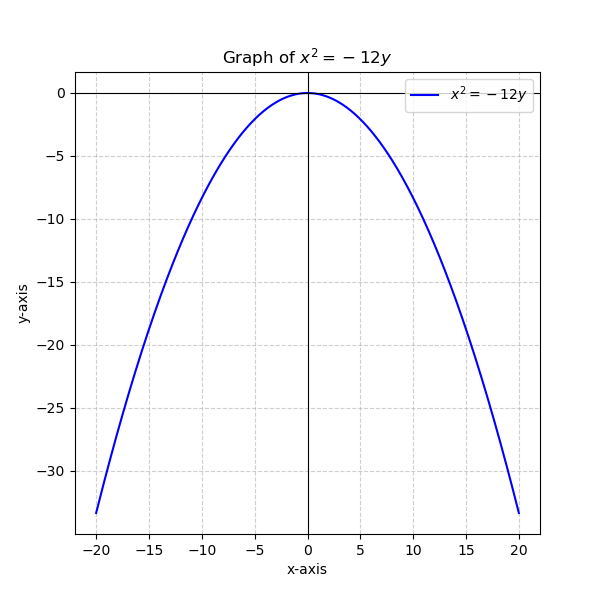
\includegraphics[width=\columnwidth, height=0.8\textheight, keepaspectratio]{Figure_14.png} 
\end{frame}
\end{document}